%%% Local Variables:
%%% TeX-command-extra-options: "-shell-escape"
%%% mode: latex
%%% TeX-master: t
%%% End:
\documentclass{beamer}
\usepackage{caption}
\usepackage{minted}
\usepackage{tikz}
\usepackage{xcolor}
\usetikzlibrary{shapes.geometric, arrows}
\tikzstyle{startstop} = [rectangle, rounded corners, minimum width=3cm, minimum height=1cm,text centered, draw=black, fill=red!30]
\tikzstyle{io} = [trapezium, trapezium left angle=70, trapezium right angle=110, minimum width=1.5cm, minimum height=0.6cm, text centered, draw=black, fill=blue!30]
\tikzstyle{process} = [rectangle, minimum width=1.5cm, minimum height=0.5cm, text centered, draw=black, fill=orange!30]
\tikzstyle{decision} = [circle, radius=2.5cm, text centered, draw=black, fill=green!30]
\tikzstyle{arrow} = [thick,->,>=stealth]
\usepackage[labelformat=simple]{subcaption}

\usetheme{Singapore}
\title{Structures and All That}
\begin{document}
\begin{frame}
\titlepage
\end{frame}
\section{Compound Data}

\begin{frame}
``Here at Brymar College\\
We can get you prepared for the 31st century\\
With advanced programming and quad rendering\\
And Java plus plus plus scripting language\\
We offer advanced job placement assistance''\\\\
from Upgrade by Deltron 3030  
\end{frame}

\begin{frame}
  \frametitle{Data Descriptions Matter}
  We have taken a weird approach by fixating on data structured in the form of ``or'' first.
  \begin{itemize}
  \item<2-> We would say that a traffic light's state is red \textbf{\emph{or}} yellow \textbf{\emph{or}} green. I will sometimes refer to data
    in this form as defining a \emph{sum type}, but for now I will stick to saying itemization.
  \item<3-> But tons of data is written in a compound manner. A person has a head \textbf{\emph{and}} a face \textbf{\emph{and}} a body ...
    I will sometimes refer to data in this form as being a \emph{product type}, but will usually stick to saying \emph{struct}.
    When I talk about classes, I will be talking about more than compound data.
  \item<4-> Whereas with ``or'' we would check which kind of data we would have and then use a computation specific to that data, with
    products we can directly project out data.
  \item<5-> Let's say that in Java that you have some person class with a first and last name represented as strings.
  \item<6-> It is easy to define a method that returns the person's full name by concatenating the first and last name.
  \end{itemize}
\end{frame}



\begin{frame}
  \frametitle{Who Needs Structs Anyway?}
  So, why do we need compound data?
  \begin{itemize}
  \item<2-> The obvious answer is that we have programs that have some kind of compound state.
  \item<3-> Consider the simple program where we wanted to move a dot left and right.
  \item<4-> We were able to represent the state of the world as a single position number.
  \item<5-> Let's add another dimension of movement where we can now move the dot up and down.
  \item<6-> Can we represent the state of the world as a single number?
  \item<7-> If you said no, I get it! But that happens to be incorrect.
  \item<8-> We can represent a grid  with one number in the same sense that we can simulate a 10x10 2D array
    with a 100 element array.
  \end{itemize}
\end{frame}

\begin{frame}
  \frametitle{Structs Make Things Easier}
  Personally, I like doing things the easy way.
  \begin{center}
    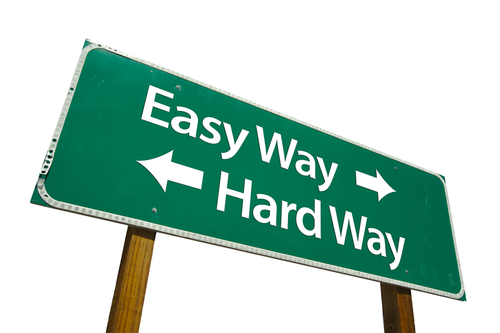
\includegraphics{images/easy-way.jpg}
  \end{center}  
\end{frame}

\defverbatim[colored]\fstName{
\begin{minted}{python}
def first_name(tup):
  return tup[0]
\end{minted}
}

\begin{frame}
  \frametitle{Unstructured Compound Data?}
  We can actually represent compound data without needing to provide names for the individual pieces of data.
  \begin{itemize}
  \item<2-> Let's consider some individual examples in Python.
  \item<3-> We can represent a Person with a first name, last name, and age with the following kind of tuple:
  \item<4-> \mintinline{python}{("Peter", "Campora", 26)}
  \item<5-> We could then define functions to act like field accesses.
  \item<6-> \fstName
  \end{itemize}
\end{frame}

\begin{frame}
  \frametitle{Data (Un)Structures}
  We can actually define other data structures in terms of things like lists.
  \begin{itemize}
  \item<2-> Let's consider defining a binary tree in terms of a python list.
  \item<3-> We can define a null node with \mintinline{python}{[]}
  \item<4-> A tree with a single root element can be \mintinline{python}{[[] 1 []]}
  \item<5-> Here's a nice balanced tree \mintinline{python}{[[[] 1 []] 2 [[] 3 []]]}
  \item<6-> This representation gets a bit ugly fast, huh?
  \item<7-> So Python gives classes (or named tuples) as a way to more easily
    define such structured data.
  \end{itemize}
\end{frame}

\begin{frame}
  \frametitle{Unstructured Data in Racket}
  Similarly, we can define data using pairs and lists in Racket.
  \begin{itemize}
  \item<2-> We can write a pair $(1, 2)$ as \mintinline{racket}{(1 . 2)}.
  \item<3-> We can write a linked list 1->2->3->4->empty as \mintinline{racket}{'(1 2 3 4)}
  \item<4-> To get the first element in the linked list, you can write:
    \mintinline{racket}{(first '(1 2 3 4))}$\hookrightarrow$ \mintinline{racket}{1}
  \item<5-> To get the rest of the linked list you can write
    \mintinline{racket}{(rest '(1 2 3 4))}$\hookrightarrow$ \mintinline{racket}{'(2 3 4)}
  \item<6-> The empty list is represented with \mintinline{racket}{'()}
    and you can check for the empty list with \mintinline{racket}{(empty? '())}
    $\hookrightarrow$ \mintinline{racket}{\#t}
  \item<7-> We will return to discussing lists in more detail later,
    since they are \emph{extremely} important.
  \item<8-> But for now, remember that we wanted to avoid the inconveniences
    given by using other existing data types to represent some piece of compound data!
  \end{itemize}
\end{frame}

\begin{frame}
  \frametitle{The Talk}
  We said that we didn't want to represent all of our compound data with
  existing structures like lists are tuples, so
  let's \emph{finally} talk about structs.
  \begin{itemize}
  \item<2-> Let's reconsider our 2 dimensional movement program.
  \item<3-> We need a natural representation for cartesian coordiantes for the state of our world.
  \item<4-> We could obviously have the state of our our world be a pair
    \mintinline{racket}{'(x . y)} or a list \mintinline{racket}{'(x  y)}
  \item<5-> But it would be better if we had piece of compound data with two fields, one field named x to represent the x coordinate and similarly a y...
  \item<6-> To define the struct: \mintinline{racket}{(struct point [x y])}
  \item<7-> To make a new point: \mintinline{racket}{(define one-two (point 1 2))}
  \item<8-> To get the x-coordinate: \mintinline{racket}{(point-x one-two)}
  \end{itemize}
\end{frame}

\defverbatim[colored]\distance{
\begin{minted}{racket}
    ;;Point -> Number
    ;;Compute a point's distance from the origin
    (define (distance-to-0 ap) 0)
\end{minted}
}

\defverbatim[colored]\distanceExamples{
\begin{minted}{racket}
    (check-expect (distance-to-0 (point 0 5)) 5)
    (check-expect (distance-to-0 (point 7 0)) 7)
\end{minted}
}

\defverbatim[colored]\distanceSkeleton{
\begin{minted}{racket}
    (define (distance-to-0 ap)
      (... (point-x ap) ...
       ... (point-y ap) ...))
\end{minted}
}

\defverbatim[colored]\distanceFinal{
\begin{minted}{racket}
    (define (distance-to-0 ap)
      (sqrt
        (+ (sqr (point-x ap))
           (sqr (point-y ap)))))
\end{minted}
}

\begin{frame}
  \frametitle{Writing Simple Programs With Structs}
  Before we consider writing more complex applications involving structs,
  let's consider writing a simple function.
  \begin{itemize}
  \item<2-> Let's consider computing the distance to the origin where we
    take in one parameter that is a point, instead of taking two parameters
    for an x-coordinate and y-coordinate.
  \item<3-> As will happen many times in this course, we will introduce
    the concept by examples before we cover how our design recipes change
    to address this new feature
  \item<4-> \distance
  \item<5->Let's add functional examples as tests:
  \item<6-> \distanceExamples
  \end{itemize}
\end{frame}

\begin{frame}
  \frametitle{Structs and Skeletons}
  We now can take inventory (step 4) and add a skeleton for our function.
  In this case we should know that we have to project out the x-coordinate
  and the y-coordinate in our distance function.
  \begin{itemize}
  \item<2-> \distanceSkeleton
  \item<3-> To code, we essentially have the same logic as when we had a previous
    version of this function that took in two parameters. Now, we just use
    the projected out x-coordinate and y-coordinate from our point.
  \item<4-> \distanceFinal
  \end{itemize}
\end{frame}

\begin{frame}
  \frametitle{Structs in General}
  Testing that function is simple, so let's just move on to talking about
  structs in general.
  \begin{itemize}
  \item<2-> You can define a struct in general with:
    \mintinline{racket}{(struct s-name [field-name-1 ...field-name-n])}
  \item<3-> After creating a struct, 3 kinds of functions are automatically
    made for you.
    \begin{enumerate}
    \item<4-> One constructor, a function that creates structure instances. It takes as many values as there are fields; as mentioned, structure is short for structure instance. The phrase structure type is a generic name for the collection of all possible instances;
    \item<5-> One selector per field, which extracts the value of the field from a structure instance; and
    \item<6-> One structure predicate, which, like ordinary predicates, distinguishes instances from all other kinds of values.
    \end{enumerate}
  \end{itemize}
\end{frame}

\begin{frame}
  \frametitle{Basic Struct Options}
  Let's illustrate each of these three kinds of functions, with our point
  struct.
  \begin{enumerate}
  \item<2-> The constructor is: \mintinline{racket}{(point x-val y-val)}
    where x-val and y-val will be values passed to the x-field and y-field in
    our point struct. The general form is \mintinline{racket}{(struct-name field-name-1-arg ... field-name-n-arg)}
  \item<3-> The selectors per field are \mintinline{racket}{(point-x point-val)} and \mintinline{racket}{(point-y point-val)}. The general form
    of a selector for a specific field is \mintinline{racket}{(struct-name-field-name val)}
  \item<4-> A predicate for checking types is automatically created, for example:
    \mintinline{racket}{(point? point-val)} and in general a predicate
    \mintinline{racket}{struct?} is created.
  \end{enumerate}
\end{frame}

\begin{frame}
  \frametitle{Examples of Structs}
  Here are some basic examples of structs:
  \begin{itemize}
  \item<2-> \mintinline{racket}{(struct movie [title producer year])}
  \item<3-> \mintinline{racket}{(struct person [name hair eyes phone])}
  \item<4-> You guys should be able to think of many more examples.
  \end{itemize}
  \pause
  \textbf{Sample Problem} Develop a structure type definition for a program that deals with “bouncing balls,”. The ball’s location is a single number, namely the distance of pixels from the top. Its constant speed is the number of pixels it moves per clock tick. Its velocity is the speed plus the direction in which it moves.
\end{frame}

\begin{frame}
  \frametitle{Designing Our Ball Struct}
  Since we are talking about a ball that bounces up and down, our structure definition is pretty simple. We need a single number for the y position and single
  number for the velocity in the y-axis.
  \begin{itemize}
  \item<2-> \mintinline{racket}{(struct ball [location vec])}
  \item<3-> This is simple because our ball is moving in a single direction. But if we had a Brick Breaker esque game then we would have a bouncing ball that
    travels along a 2D plane, then our definition is much more complicated.
  \item<4-> Let's first consider defining a 2D vector struct as follows: \mintinline{racket}{(struct vector [delta-x delta-y])}
  \item<5-> Now, we can represent a ball as a point (which only has positive components) and a vector (which can have negative components):
    \mintinline{racket}{(struct 2D-ball position vec)}
  \end{itemize}
\end{frame}

\defverbatim[colored]\pointDefinition{
\begin{minted}[fontsize=\footnotesize]{racket}
    (define-struct point [x y])
    ; A Point is a structure: 
    ;   (point Number Number)
    ; interpretation a point x pixels from left, y from top
\end{minted}
}

\begin{frame}
  \frametitle{Other Representations}
  Our 2D Ball struct has nested occurrences of other structs. This is a natural thing, and even recursive descriptions of data are natural, i.e.
  linked lists and binary trees. But we can also consider using a \emph{flat representation} for our 2D Ball, which doesn't nest structs.
  \begin{itemize}
  \item<2-> \mintinline{racket}{(struct 2D-ball [x y delta-x delta-y]}
  \item<3-> Although valid, I think it's better to keep representations natural and just nest things, barring performance concerns.
  \item<4-> Let's talk about defining data definitions for structs. We must specify the form of the struct and the types of its field and provide an interpretation of what
    each of the fields represents. Here's how we do this for our point struct:
  \item<5->\pointDefinition
  \end{itemize}
\end{frame}

\defverbatim[colored]\moveDotStart{
\begin{minted}{racket}
(define MTS (empty-scene 100 100))
(define DOT (circle 3 "solid" "red"))
 
; A Point represents the state of the world.
 
; Point -> Point
(define (main p0)
  (big-bang p0
    [on-tick x+]
    [on-mouse reset-dot]
    [to-draw scene+dot]))   
\end{minted}
}

\begin{frame}
  \frametitle{Structs and Program Design}
  Now we need to consider designing programs using structs.
  \textbf{Sample Problem} Your team is designing an interactive game program that moves a red dot across a image canvas and allows players to use the mouse to reset the dot. Here is how far you got together: \pause
  \moveDotStart
\end{frame}

\defverbatim[colored]\sceneDotHeader{
\begin{minted}{racket}
    ; Point -> Image
    ; adds a red spot to MTS at p
    (define (scene+dot p) MTS)
\end{minted}
}

\defverbatim[colored]\sceneDotExamples{
\begin{minted}{racket}
    (check-expect (scene+dot (point 10 20))
                  (place-image DOT 10 20 MTS))
    (check-expect (scene+dot (point 88 73))
                  (place-image DOT 88 73 MTS))

\end{minted}
}

\defverbatim[colored]\sceneDotSkeleton{
\begin{minted}{racket}
    (define (scene+dot p)
      (... (point-x p) ... (point-y p) ...))
\end{minted}
}

\begin{frame}
  \frametitle{Designing scene+dot}
  Let us first assume that you're tasked with designing \mintinline{racket}{scene+dot}.
  \begin{itemize}
  \item<2-> Of course, we already have our data interpretation so we start
    with step 2 and provide our signature, statement of purpose, and
    function header.
  \item<3-> \sceneDotHeader
  \item<4-> Finishing step 3 and creating the following functional examples (as tests) is straightforward:
  \item<5-> \sceneDotExamples
  \end{itemize}
\end{frame}

\defverbatim[colored]\sceneDotFinal{
\begin{minted}{racket}
    (define (scene+dot p)
      (place-image DOT (point-x p) (point-y p) MTS))
\end{minted}
}

\begin{frame}
  \frametitle{Designing scene+dot (cont.)}
  We can now move on to carrying out step 4 and taking inventory:
  \begin{itemize}
  \item<2-> \sceneDotSkeleton
  \item<3-> Finishing step 5 is easy, we simply need to place the
    projected x and y coordinates as arguments to \mintinline{racket}{place-image}
  \item<4-> \sceneDotFinal
  \item<5-> Testing this is uninteresting, so let's consider if we were asked
    to define the \mintinline{racket}{x+} function, which takes in a Point
    and returns a new Point with an x-coordinate that is 3 units further to
    the right of the old point.    
  \end{itemize}
\end{frame}

\defverbatim[colored]\xPlusHeader{
\begin{minted}{racket}
    ;;Point -> Point
    ;;Updates the position of our dot at each clock tick
    (define (x+ p) p)
\end{minted}
}

\defverbatim[colored]\xPlusExamples{
\begin{minted}{racket}
    (check-expect (x+ (point 0 0)) (point 3 0))
    (check-expect (x+ (point 10 10)) (point 13 10))
    (check-expect (x+ (point 0 10)) (point 3 10))
\end{minted}
}

\defverbatim[colored]\xPlusSkeleton{
\begin{minted}{racket}
    (define (x+ p) (... (point-x p) ... (point-y p) ...)
\end{minted}
}

\begin{frame}
  \frametitle{Designing x+}
  Designing our  \mintinline{racket}{x+} function is a bit harder than
  \mintinline{racket}{scene+dot}, because we are producing structures
  as output.
  \begin{itemize}
  \item<2-> When carrying out step 2, recall that \mintinline{racket}{x+} handles clock ticks:
    \xPlusHeader
  \item<3-> Coming up with functional examples as tests is
    straightforward:
    \xPlusExamples
  \item<4-> To take inventory we project out the x and y fields
    from our point, as usual:
    \xPlusSkeleton
  \end{itemize}
\end{frame}

\defverbatim[colored]\xPlusFinal{
\begin{minted}{racket}
    (define (x+ p)
      (point (+ (point-x p) 3) (point-y p)))
\end{minted}
}

\begin{frame}
  \frametitle{Designing x+ (cont.)}
 To finish coding, we need to first add 3 to the x-coordinate
 and then pack the result back into a new point structure.
 \begin{itemize}
 \item<2-> \xPlusFinal
 \item<3-> This is a perfect example of the \emph{essence} of
   functional programming. We are creating a \emph{new} point
   whose x-coordinate is based on the old one, instead of modifying
   the original point to store a new x-coordinate.
 \item<4-> But there is something inelegant about this, right?
 \item<5-> If we had more fields than y, we simply are projecting
   out the old field as an argument when creating the new struct
   value.
 \item<6-> This adds a lot of boilerplate code...
 \end{itemize}
\end{frame}

\defverbatim[colored]\pointSet{
\begin{minted}{racket}
    (define (point-set-x p x)
      (point x (point-y p))
\end{minted}
}

\defverbatim[colored]\xPlusNew{
\begin{minted}{racket}
    (define (x+ p)
      (point-set-x p (+ (point-x p) 3)))
\end{minted}
}

\begin{frame}
  \frametitle{Struct Boilerplate}
  We might want to define a function, \mintinline{racket}{point-set-x} which takes in a point and a value
  and produces a new point where the x-coordinate is the given value and the y-coordinate is taken from the old point.
  \begin{itemize}
  \item<2-> Here is the code: \pointSet
  \item<3-> We can now redefine \mintinline{racket}{x+} with it:
    \xPlusNew
  \item<4-> \mintinline{racket}{point-set-x} is  known as
    a \emph{functional setter}, similar to a more traditional setter
    in languages like Java.
  \item<5-> However, defining an update operation on a complicated
    structure can get very complicated, and we can get around
    this uses \emph{lenses} (we may discuss this later in the course).
  \end{itemize}
\end{frame}

\end{document}



%%% Local Variables:
%%% TeX-command-extra-options: "-shell-escape"
%%% mode: latex
%%% TeX-master: t
%%% End:
